\documentclass[12pt,a4paper]{article}
\usepackage[utf8]{inputenc}
\usepackage[german]{babel}
\usepackage[T1]{fontenc}
\usepackage{amsmath}
\usepackage{amsfonts}
\usepackage{amssymb}
\usepackage{graphicx}
\usepackage[left=2cm,right=2cm,top=2cm,bottom=2cm]{geometry}
\author{Tim}

\begin{document}

\tableofcontents
\newpage

\section{Prismenspektrometer}

\subsection{Grundlagen}

\subsection{Dispersionskurve}
In diesem Teilversuch wurde die Dispersionskurve des verwendeten Prismas mithilfe einer Quecksilber-Cadmium-Lampe vermessen.

\subsection{Dispersionskurve}
In diesem Teilversuch wurde die Dispersionskurve des verwendeten Prismas mithilfe einer Quecksilber-Cadmium-Lampe vermessen.

\subsubsection{Aufbau und Durchführung}
Durch eine Kollimatorlinse werden ebene Wellenfronten erzeugt. Diese werden mit dem einem Drehteller befindlichen Prisma gebrochen. Das gebrochene Spaltbild wird mit einem schwenkbaren Fernrohr beobachtet. Die relative Position des Fernrohrs kann dabei auf 1' genau abgelesen werden.

In diesem Versuch werden zunächst die Minimalablenkungen des Prismas für mehrere Spektrallinien bestimmt.
Durch gleichsinniges Drehen von Prismenteller und Fernrohr wandern auch die Spektrallinien, zunächst in die eine und dann in die andere Richtung. Der Umkehrpunkt entspricht dabei der Minimalablenkung. Man wiederholt die Messung, diesmal trifft das Licht allerdings auf der anderen Prismenseite auf. Dann gilt für die Minimalablenkung

\begin{equation}
2 \delta_{min} = \psi_2-\psi_1
\end{equation}

wobei $\psi_i$ die Umkehrpunkte sind.
Zur Bestimmung der statistischen Unsicherheit auf die $\psi_i$ wurde eine Rauschmessung an der $\psi_1$-Position der blau-grünen Cadmiumlinie ($\lambda=508,58nm$) durchgeführt.

Für die übrigen Positionen der Spektrallinien wurde die Messung drei (bzw. fünf) mal wiederholt. Der Fehler auf die sich so ergebenden Mittelwert ist dann $\sigma_{\psi}=\frac{\sigma_{psi}}{\sqrt{N}}$.

Es ergeben sich damit die Minimalablenkungen und der Fehler auf selbige für jede vermessene Spektrallinie.

\begin{equation}
\sigma_{\delta} = \sqrt{\sigma_{\psi_1}^2+\sigma_{psi_2}^2}
\end{equation}

Damit folgt für die Brechungsindizes bei den entsprechenden Wellenlängen::

\begin{equation}
n = \frac{sin(\frac{\delta_{min}+\epsilon}{2})}{sin(\frac{\epsilon}{2})}
\end{equation}

\begin{equation}
\sigma_n = \frac{cos(\frac{\delta_{min}+\epsilon}{2})}{sin(\frac{\epsilon}{2})} \frac{\delta_{min}}{2}
\end{equation}

\subsubsection{Rohdaten}

\begin{table}
\begin{center}
\begin{tabular}{|c|c|}
\hline 
$\psi_1$ & $\psi_2$ \\ 
\hline 
25$^{\circ}$3' & 147$^{\circ}$21' \\ 
\hline 
25$^{\circ}$1' & 147$^{\circ}$22' \\ 
\hline 
25$^{\circ}$0'& 147$^{\circ}$13' \\ 
\hline 
25$^{\circ}$1' & 147$^{\circ}$11' \\ 
\hline 
25$^{\circ}$1' & 147$^{\circ}$16' \\ 
\hline 
25$^{\circ}$3' & \\ 
\hline 
25$^{\circ}$9' & \\ 
\hline 
25$^{\circ}$3' & \\ 
\hline 
25$^{\circ}$10' & \\ 
\hline 
25$^{\circ}$20' & \\ 
\hline 
25$^{\circ}$14' & \\ 
\hline 
25$^{\circ}$11' & \\ 
\hline 
25$^{\circ}$9' & \\ 
\hline 
25$^{\circ}$8' & \\ 
\hline 
25$^{\circ}$10' & \\ 
\hline 

\end{tabular} 
\label{tab:RauschenPrisma}
\caption{Rohdaten der grün-blauen Cadmiumlinie. Die Messwerte auf $\psi_1$ dienen als Rauschmessung für die statistische Unsicherheit .}
\end{center}
\end{table}


\begin{table}
\begin{center}
\begin{tabular}{|c|c|}
\hline
$\psi_1$ & $\psi_2$ \\
\hline
$\lambda =$404.66nm & \\
\hline
21$^{\circ}$2' &151$^{\circ}$15' \\
\hline
21$^{\circ}$0' &151$^{\circ}$14' \\
\hline
20$^{\circ}$56' &151$^{\circ}$18' \\ 
\hline
$\lambda =$435.83nm & \\
\hline
22$^{\circ}$43' &149$^{\circ}$34' \\
\hline
22$^{\circ}$45' &149$^{\circ}$33' \\ 
\hline
22$^{\circ}$42' &149$^{\circ}$33' \\ 
\hline
$\lambda =$467.81nm & \\
\hline
23$^{\circ}$55' &148$^{\circ}$22' \\
\hline
23$^{\circ}$54' &148$^{\circ}$24' \\
\hline
23$^{\circ}$57' &148$^{\circ}$20' \\ 
\hline
$\lambda =$479.99nm & \\
\hline
24$^{\circ}$22' &147$^{\circ}$56' \\ 
\hline
24$^{\circ}$24' &148$^{\circ}$0' \\ 
\hline
24$^{\circ}$18' &148$^{\circ}$2' \\ 
\hline
$\lambda =$564.07nm & \\
\hline
25$^{\circ}$53' &146$^{\circ}$24' \\
\hline
25$^{\circ}$54' &146$^{\circ}$25' \\
\hline
25$^{\circ}$54' &146$^{\circ}$22' \\ 
\hline
$\lambda =$579.07nm & \\
\hline
26$^{\circ}$34' &145$^{\circ}$48' \\
\hline
26$^{\circ}$32' &145$^{\circ}$44' \\
\hline
26$^{\circ}$33' &145$^{\circ}$44' \\ 
\hline
$\lambda =$643.85nm & \\
\hline
27$^{\circ}$20' &144$^{\circ}$57' \\
\hline
27$^{\circ}$20' &144$^{\circ}$55' \\
\hline
27$^{\circ}$24' &144$^{\circ}$59' \\
\hline
\end{tabular}
\label{tab:RohdatenDispersion}
\caption{Rohdaten für die Position der beiden Umkehrpunke für die vermessenen Spektrallinien der HgCa-Lampe. Die Wellenlängen sind dem Praktikumsskript (S.19) entnommen worden.}
\end{center}
\end{table}

Das Ergebnis der Rauschmessung zur Bestimmung des statistischen Fehlers für die Winkelmessung findet sich in Tabelle \ref{tab:RauschenPrisma}.
Die Rohdaten der restlichen Spektrallinien, welche Vermessen wurden sind in Tabelle \ref{tab:RohdatenDispersion} dargestellt.


\subsubsection{Auswertung}

\begin{table}
\begin{center}
\begin{tabular}{|c|c|c|}
\hline
$\lambda /nm$ & $\delta_{min} / rad$ & n \\
\hline
404.66 & 1.1368 $\pm$ 0.0007 & 1.7751$\pm$ 0.0004\\
\hline
435.83 & 1.1068$\pm$ 0.0007 & 1.7611$\pm$ 0.0004\\
\hline
467.81 & 1.086$\pm$ 0.0007 & 1.7511$\pm$ 0.0004\\
\hline
479.99 & 1.0789$\pm$ 0.0007&1.7477$\pm$ 0.0004\\
\hline
508.58 & 1.0661$\pm$ 0.0004 & 1.7414$\pm$ 0.0002\\
\hline
546.07 & 1.0516$\pm$ 0.0007 & 1.7342$\pm$ 0.0004\\
\hline
579.07 & 1.0403$\pm$ 0.0007 & 1.7286$\pm$ 0.0004\\
\hline
643.85 & 1.0262$\pm$ 0.0007 & 1.7215$\pm$ 0.0004\\
\hline
\end{tabular}
\label{tab:AuswertungDispersion}
\caption{Ergebnisse der Auswertung. Dargestellt ist der bestimmte minimale Ablenkungswinkel mit Unsicherheit für jede vermessene Linie sowie die sich daraus ergebenden Brechungsindizes.}
\end{center}
\end{table}

\begin{figure}
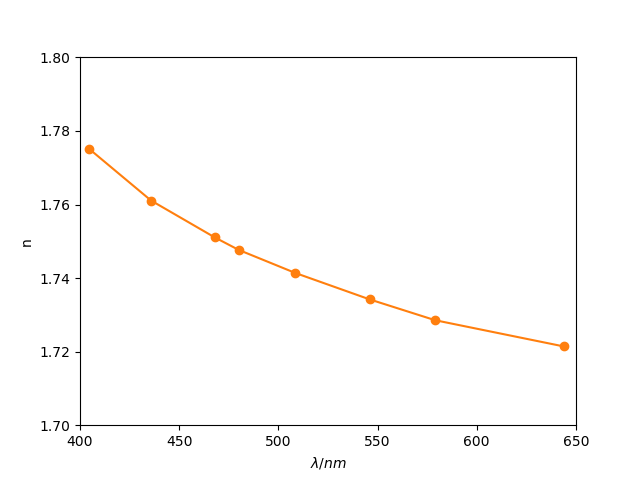
\includegraphics[scale=1.0]{Bilder/Dispersionskurve.png}
\label{fig:Dispersionskurve}
\caption{Die Dispersionskurve des verwendeten Prismas. Die Fehlerbalken auf die n-Werte sind relativ klein und somit nicht erkennbar. Die einzelnen Messpunkte wurden zur Veranschaulichung verbunden.}
\end{figure}

\begin{figure}
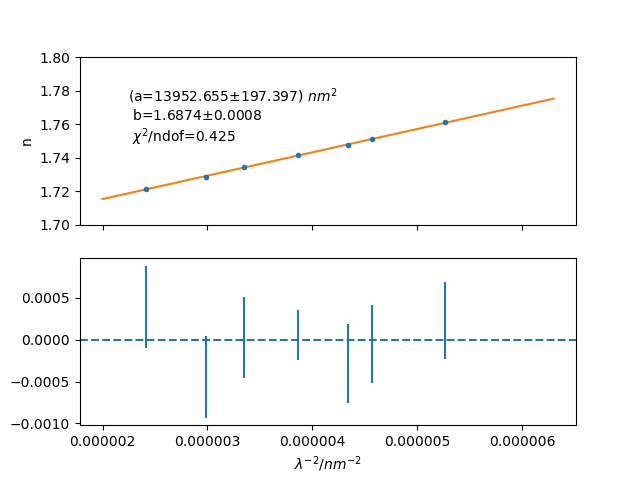
\includegraphics[scale=1.0]{Bilder/Regression.png}
\label{fig:RegressionDispersion}
\caption{Auftragung von n gegen $1/\lambda^2$. Das beste Anpassung ergab sich für eine Anpassungsgerade der Form $n(\lambda) = \frac{a}{\lambda^2} + b $}. Auch hier sind die Fehlerbalken aufgrund der geringen Größe kaum erkennbar.
\end{figure}


Die Rauschmessung ergibt eine statistische Unsicherheit auf die $\psi_i$ von $\sigma_{\psi_i} = 0.0017 rad$ bzw. $\sigma_{\psi_i} = 5.8'$. Wie in der Durchführung beschrieben kann nun aus den Daten die Minimalablenkung $\delta_{min}$ und der entsprechende Fehler, sowie aus diesen der Brechungsindex und seine Unsicherheit für die entsprechenden Wellenlängen berechnet werden.
Die Werte sind in Tabelle \ref{tab:AuswertungDispersion} dargestellt.

Durch Auftragen des Brechungsindex gegen die Wellenlänge erhält man die Dispersionskurve (Abb. \ref{fig:Dispersionskurve}).




\newpage
\section{Gitterspektrometer}

\subsection{Grundlagen}
Ein Gitter ist ein optisches Bauteil, das einfallendes Licht beugt. Das Beugungsmuster ist ähnlich dem der Beugung an einem Doppelspalt. Allerdings hat das Gitter gegenüber dem Doppelspalt einige Vorteile: Durch die hohe Anzahl der Spalte ist die durchgelassene Intensität deutlich höher als bei einem Doppelspalt. Zudem ermöglicht dies schmalere Spalte, welches eine besser Auflösung ermöglicht.

\subsection{Aufbau und Durchführung}

\subsection{Bestimmung der Gitterkonstanten}

\subsection{Bestimmung der Wellenlänge}

\subsection{Bestimmung der Auflösung}

\subsection{Zusammenfassung}


\end{document}